\chapter{Camera Sensing and Integration into the World Frame for a Pick and Place Task}

\section{Important}
Read the entire lab before starting and especially the "Grading" section as there are points you will receive by completing certain sections or checkpoints
by the end of the lab session(s). 
\section{Objectives}
This is the capstone lab of the semester and will integrate your work done in previous labs with python, ROS, forward and inverse kinematics and OpenCV.  In this lab you will:
\begin{itemize}
	\item Use OpenCV functions to find the centroid of each colored block and draw crosshair at that centroid along with a circle around the object.
	\item Develop transformation equations that relate pixels in the image to coordinates in the world frame
	\item Report the world frame coordinates $(x_w,y_w)$ of the centroid of each block in the camera’s view.
	\item Sort the two colors of blocks to predefined positions in the robot's work area.
\end{itemize}

\section{References}
\begin{itemize}
	\item Review the vision setup and processing parts of Lab 3 as many items will be repeated here in Lab 6.
	\item Re-visit Appendix C which explains how to simplify the intrinsic and extrinsic equations for the camera.
    \item HSV Color Space:
    \begin{itemize}
    \item \url{https://en.wikipedia.org/wiki/HSL_and_HSV}
    \item \href{https://stackoverflow.com/questions/10948589/choosing-the-correct-upper-and-lower-hsv-boundaries-for-color-detection-withcv}{https://stackoverflow.com/questions/10948589/}
    \end{itemize}
    
    \item Simple Blob detector:
    \begin{itemize}
    \item \url{www.learnopencv.com/blob-detection-using-opencv-python-c/}
    \item \href{https://stackoverflow.com/questions/8076889/}{https://stackoverflow.com/questions/8076889/how-to-use-opencv-simpleblobdetector}
    \item \url{https://www.programcreek.com/python/example/89350/cv2.SimpleBlobDetector}
    \item \url{https://www.programcreek.com/python/example/71388/cv2.SimpleBlobDetector_Params}
    \end{itemize}

\end{itemize}



\section{Tasks}
\subsection{Color Thresholding and Object Centroids}
In the same way you used the HSV color space in Lab3 to find the orange color, find HSV ranges to identify both bright pink and bright green blocks.  Then use \textbf{OpenCV} library functions to locate the centroid of the four blocks placed in the camera's view.  In Lab 3, you were required to use the \textbf{SimpleBlobDectector} class to find the orange circle’s centroid.  Here in Lab 6, you can again use the \textbf{SimpleBlobDectector} class to find all the block’s centroids, but if you would like to experiment with other OpenCV function, you are encouraged to do so.

\subsection{Camera Setup}
The problem of camera setup is that of relating (row,column) coordinates in an image to the corresponding coordinates in the world frame $(x_w,y_w,z_w)$. For our purposes we may make several assumptions that will vastly simplify camera calibration. Please consult Appendix C and follow along with the simplification of the general equations.

Several parameters must be specified in order to implement the equations. Specifically, we are interested in \textbf{$\theta$} the rotation between the world frame and the camera frame and \textbf{$\beta$} the scaling constant between distances in the world frame and distances in the image. We will compute these parameters by measuring object coordinates in the world frame and relating them to their corresponding coordinates in the image.

\subsection{Pick and Place}
Your program should:

\begin{itemize}
\item Move the Robot out of the way so that the camera can view Lab 3's entire grid area in order to find the blocks randomly placed in that area.  

\item Use \textbf{OpenCV} functions to find the centroid $(x_w,y_w)$ of each block.

\item Display a center point and a circle around each discovered block in the video display window.  

\item Command the robot to pick up each block one at a time and place it in the green predefined positions or the pink predefined positions. 

\item When finished with all blocks exit from the program.  

\end{itemize}

\section{Procedure}
\subsection{Threshold camera image to distinguish the colors of choice} \label{ObjCentriod}

Note the below procedure in section \ref{ObjCentriod}, \ref{useOpenCV} and \ref{CamCal} is very similar to lab3 and uses lab3 files.

\begin{enumerate}
 
\item Return to your lab3 directory and run:

\begin{lstlisting}[language=bash]
$ source devel/setup.bash
$ roslaunch ur3_driver vision_driver.launch
\end{lstlisting}

Open a second terminal window

\begin{lstlisting}[language=bash]
$ source devel/setup.bash
$ rosrun lab3pkgpy lab3_image_tf_exec.py
\end{lstlisting}

You should see two Windows open.  One is the camera’s video with an added horizontal black line and small red circle.  Later in this lab you will use the horizontal line to straighten the mounting of the camera if it got moved or bumped.  For the red dot towards the top left corner of the image look at the text printing in the terminal.  A three number (H,S,V) value is printing.  You can use this pixel value to help you find the range of H,S,V (Hue, Saturation, Value) values for three colors. First the same orange color you found in lab3 so you can use the calibration stick to help setup your camera. Then in addition, you should find the H,S,V range for the bright pink and green blocks.

\textbf{Side Note:}  What is the H,S,V color space?  Please see the reference link to the Wikipedia  page discussing color spaces.  You are probably most familiar with the R,G,B (red,green,blue) color space.  Here each pixel of an image has a R,G,B value.  With H,S,V, colors are placed on a color wheel and you indicate which color you are interested in by selecting an angle range.  In \textbf{OpenCV} the range of the angle is from 0 degrees to 180 degrees.  (You will find other implementations that use 0-360).  For example a blueish color would be in the angle range of 110 degrees to 130 degrees.  The S value is a number between 0 and 255 with 0 being very white and washed out and 255 the full, clear color.  The V value is also a number between 0 and 255 with 0 being very dark and shaded and 255 the full clear color.  The main reason we use the H,S,V color space in this lab is that it makes finding a color with different shading and lighting conditions much easier. 

\item At this point take a look at the given python files in the \textbf{lab3pkg\_py/scripts} folder. This section will only be modifying the files \textbf{lab3\_func.py} and \textbf{lab3\_image\_tf\_exec.py}.  Take a look at these two files.  Notice in \textbf{lab3\_func.py}, in the function \textbf{blob\_search}, the code is converting the RGB image to HSV.  Then, leaving off where you ended in lab3, using a range for orange pixels the \textbf{inRange} function is used to threshold/mask the image to a binary image of only orange pixels. (Binary image means all orangeish pixels are ones and all other pixels are zeros).  Next the masked image is cropped to only use the portion of the image that views the grid.  (You will adjust the size of this cropped image in a few steps).  Then at the bottom of the function both the color image and the cropped binary image are displayed in separate windows.  (Notice in those windows there is a button that allows you to save the current image to a file.)
  
\item So your first goal is to find the 3 ranges of Hue, Saturation and Value that allows your program to find the orange calibration stick, and the pink and green blocks in the robot's work area from the camera's view.  To find these HSV ranges you will need to do some trial and error.  You are supplied with two tools to help you find the correct range.  One is the red dot printed for you on the camera’s video frames.  Notice that when you put a colored block or the orange circle under that red dot the terminal window prints out the H,S,V value for that pixel.  Experiment with a few colors and see the H,S,V values change.  The code for putting this red dot on the image and displaying the H,S,V values to the terminal is in the \textbf{lab3\_func.py} file towards the end of the \textbf{blobsearch} function.  The \textbf{cv2.circle} function is used to add the red dot and the print statement prints out the H,S,V values.   
One issue with this method is that it only shows one pixel and therefore only one lighting condition.  You need to make sure your range of H, S, V values work in all areas of the cropped image.  So going on from here, you need to do some trial and error.  Pick a range for H and S and V, change your code with that range and see how well the cropped image shows only the orange disk, and the pink or green blocks in all of its area.  We have also supplied you with some off line code, \textbf{HSV.py}, that takes a single picture file and prints out a H,S,V range for the pixels selected.   

	\begin{figure}[h]
	\centering
		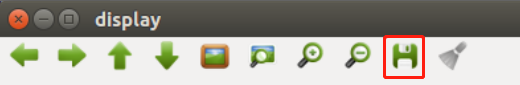
\includegraphics[height=1cm]{lab3_cam_cali7.png}
	\caption{\figlbl{3cali7} How to snapshot the video feed.}
    \end{figure}

\item Once you have found good H,S,V ranges for orange calibration stick, and the pink and green blocks and your benches lighting conditions, you need to make sure the cropped image views all the area of the grid.  First step is to look at the full color image and make sure the camera is turned so the black horizontal line is also horizontal with respect to the robot’s base.  Have your TA help you with this.  (Of course try your best not to bump the camera so that this process does not have to happen too often.).  Then return to looking at the cropped binary image and move the blocks to all corners of the grid.  Make sure that the blocks are seen in the cropped image at all the corners.  If the cropped image does not see all corners of the grid you will need to modify the values \textbf{crop\_top\_row}, \textbf{crop\_bottom\_row}, \textbf{crop\_top\_col} and \textbf{crop\_bottom\_col} to move where the top and bottom corners of the cropped image are located.  Note that the full image size is 480 rows by 640 columns. (If you have to change \textbf{crop\_top\_row}, \textbf{crop\_bottom\_row}, \textbf{crop\_top\_col} and \textbf{crop\_bottom\_col}, make a note to change these also in your lab6 code later in section \ref{PickPlace}.)

\end{enumerate}

\subsection{Use the OpenCV simpleBlobDetector library function to find the centroids of 2 Pink and 2 Green Blocks} \label{useOpenCV}

\begin{enumerate}

\item The steps below show how to use \textbf{simpleBlobDetector} to find the centroids. First you will find the centroid of the orange color to prepare for setting up the camera. Then in section \ref{PickPlace} you will change this code to look for pink, then green blocks.

You are given starter code to get you started with \textbf{simpleBlobDetector}.  See in \textbf{lab3\_func.py} the function \textbf{blob\_search\_init}.  This is where you need to set the parameters for \textbf{simpleBlobDetector} (hopefully already done in lab3).  By default all the “filterBy…” parameters are set to False.  You need to decide which of these filters will work best to find the orange disks in the cropped image.  There are also other parameters you will need to set in this function which are not given to you.  Once you think you have set all the correct parameters, switch to the \textbf{blob\_search} function and find the comment that shows you where to call the “detect” method of \textbf{simpleBlobDetector}.  

The detect method returns \textbf{keypoints}, which is a variable that has the centroid and other information of each blob found.  If there is only one block with certain color then \textbf{keypoints} only has one element.  If there are more blobs then \textbf{keypoints} also has the centroids for those blobs.  The web pages listed in the References section show example code of getting information out of the \textbf{keypoints} variable.  Use the \textbf{print()} function to print out the number of blobs found and the coordinates of the first blob.  Also use the \textbf{cv2.drawKeypoints()} function to draw a circle around each blob in the color video frames. \textbf{simpleBlobDetector} is being passed the cropped image.  The centroid found is in pixel units.  (0, 0) is the top left corner of the cropped image.  Therefore you will need to add \textbf{crop\_top\_row} and \textbf{crop\_top\_col} to the \textbf{Keypoint}'s centroid values before calling the \textbf{cv2.drawKeypoints()} function with the full color image.  \textbf{Keypoints} is a list of the \textbf{Keypoint} class.  One of the elements in the \textbf{keypoint} class is pt, which is a tuple.  To modify an element in a tuple, first change the tuple to a list with the \textbf{list()} function.  Modify the element of the newly created list and finally set the \textbf{Keypoint.pt} tuple element to the modified list by converting the list to a tuple with the \textbf{tuple()} function. Figuring out the correct parameters for \textbf{simpleBlobDetector} will take some trial and error.

\item Using the orange calibration stick, move them to many different locations in the maze and print out the centroids found.  Make sure that these centroids make sense in pixels where the (0, 0) camera origin is the top left corner. 

\end{enumerate}


\subsection{Camera Setup} \label{CamCal}
Again, a repeat of lab3 procedure:
\begin{enumerate}
    \item Read Appendix C.3 before proceeding further.
\begin{figure}[h]
	\centering
		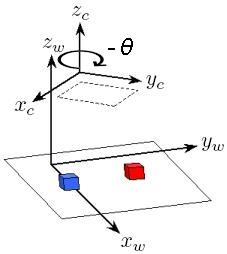
\includegraphics[height=6cm]{lab3_calibrate1.jpg}
	\caption{\figlbl{3cali1} Arrangement of the world and camera frames.}
\end{figure}

	\item Begin by writing the equations we must solve in order to relate image and world frame coordinates.  You will need to combine the 
intrinsic and extrinsic equations for the camera; these are given in Appendix C.3.  Write equations for the world frame coordinates in terms of the image coordinates.
	\begin{eqnarray*}
		x_w(r,c) & = & \\
		y_w(r,c) & = &
	\end{eqnarray*}
	
	\item There are six unknown values you must determine: $O_r, O_c, \beta, \theta, T_x, T_y$.  The principal point $(O_r,O_c)$ is given by the row and column coordinates of the center of the image.  We can easily find these values by dividing the \texttt{width} and \texttt{height} variables by 2.
	\begin{eqnarray*}
		O_r & = & \frac{1}{2}height = \\
		O_c & = & \frac{1}{2}width =
	\end{eqnarray*}
	
	\begin{figure}[h]
	\centering
		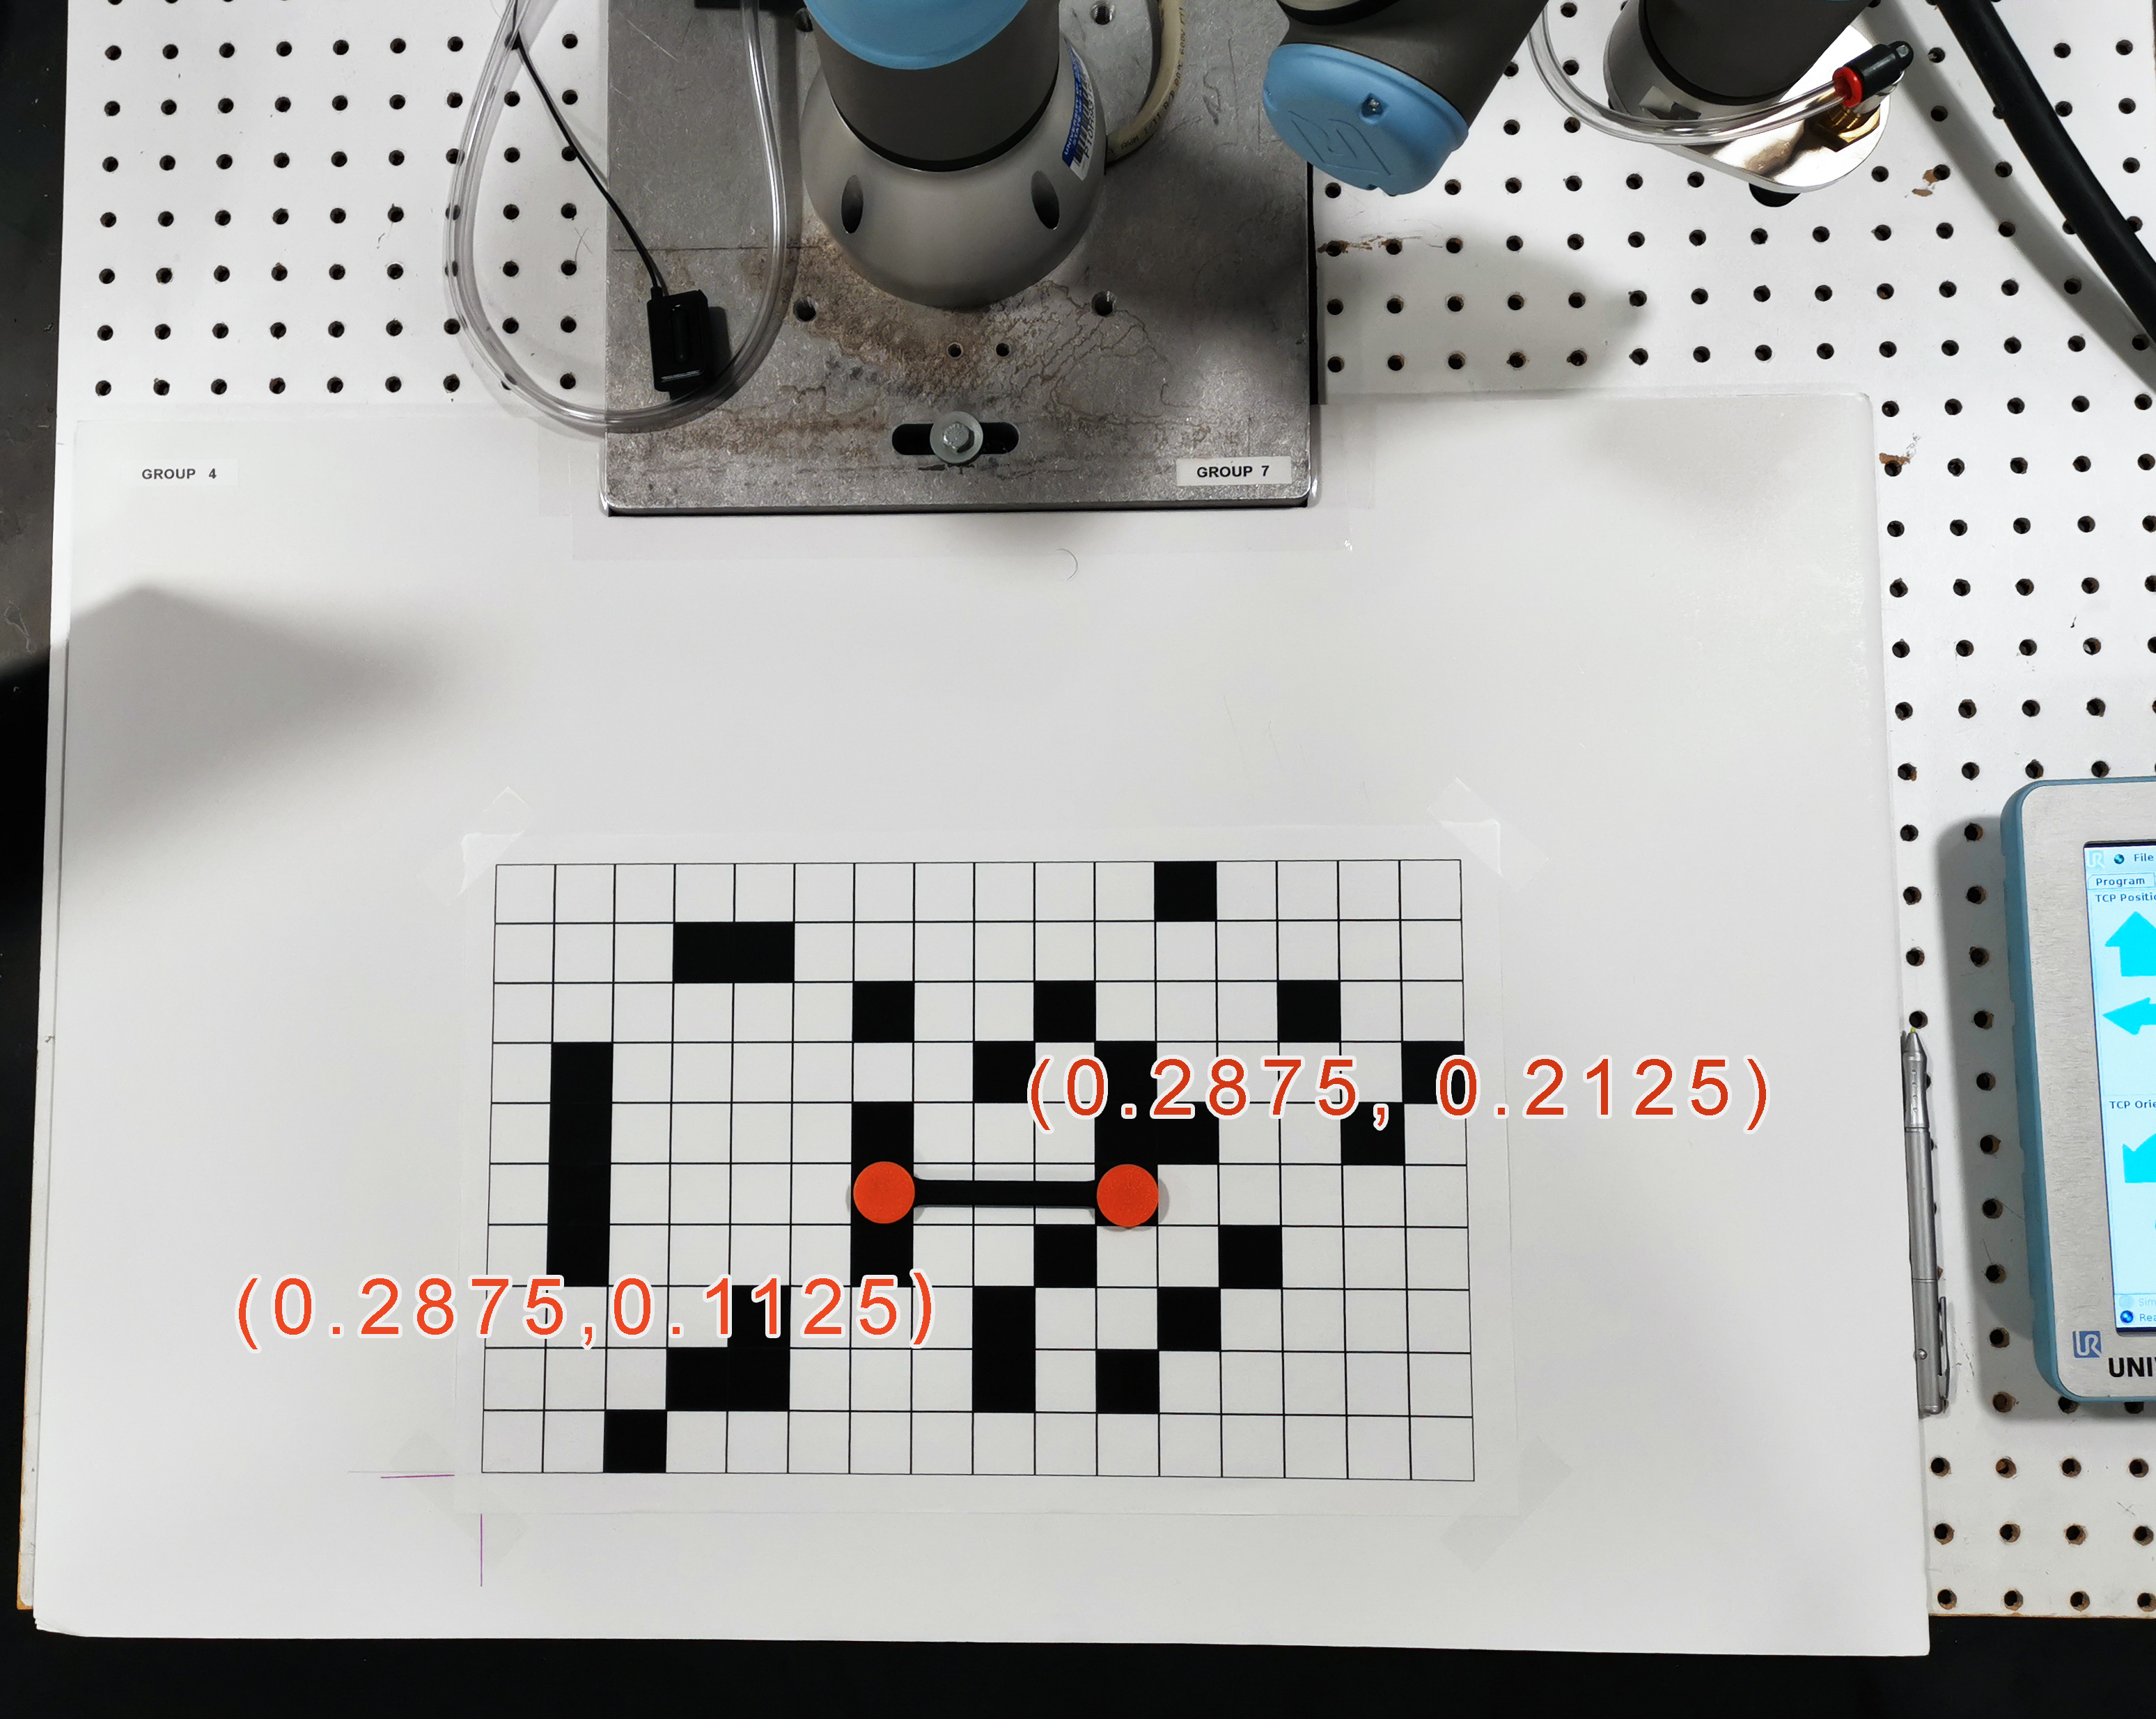
\includegraphics[height=8cm]{lab3_cam_cali6.jpg}
	\caption{\figlbl{3cali6} Where to place the calibration stick.}
    \end{figure}
	
	You will calculate the parameters $\beta, \theta, T_x, T_y$ in the python script:
	
	\textbf{lab3\_image\_tf\_exec.py}
	
	First, place the calibration stick in the position ($x_w = 0.2875$, $y_w = 0.1125$ and $x_w = 0.2875$, $y_w = 0.2125$) shown in the \figref{3cali6}. Please keep anything orange (including your hands) away from the camera's field of view. 
	Open a terminal window:
	
	\begin{lstlisting}[language=bash]
    $ source devel/setup.bash
    $ roslaunch ur3_driver vision_driver.launch
    \end{lstlisting}
    
    Open a second terminal window:
    
    \begin{lstlisting}[language=bash]
    $ source devel/setup.bash
    $ rosrun lab3pkgpy lab3_image_tf_exec.py
    \end{lstlisting}
	
    You will modify this code (which will print these values to the terminal by default as zeros) to calculate $\beta, \theta, T_x, T_y$ values so that you can use them in \textbf{lab6\_image\_exec.py}.
	
	Note that you may have to rerun this procedure to obtain these values when you return to the lab, as other groups will be using the same camera and may re-position the camera when you are not present. To keep these values relatively consistent, \textbf{PLEASE TRY NOT TO BUMP OR MOVE THE CAMERA.}
	
	$\beta$ is a constant value that scales distances in space to distances in the image.  That is, if the distance (in unit length) between two points in space is $d$, then the distance (in pixels) between the corresponding points in the image is $\beta d$. Note that the calibration stick is exactly 0.1 m long.
	\[
	\beta =
	\]
	
    \begin{figure}[t]
	\centering
	\begin{tabular}{cc}
		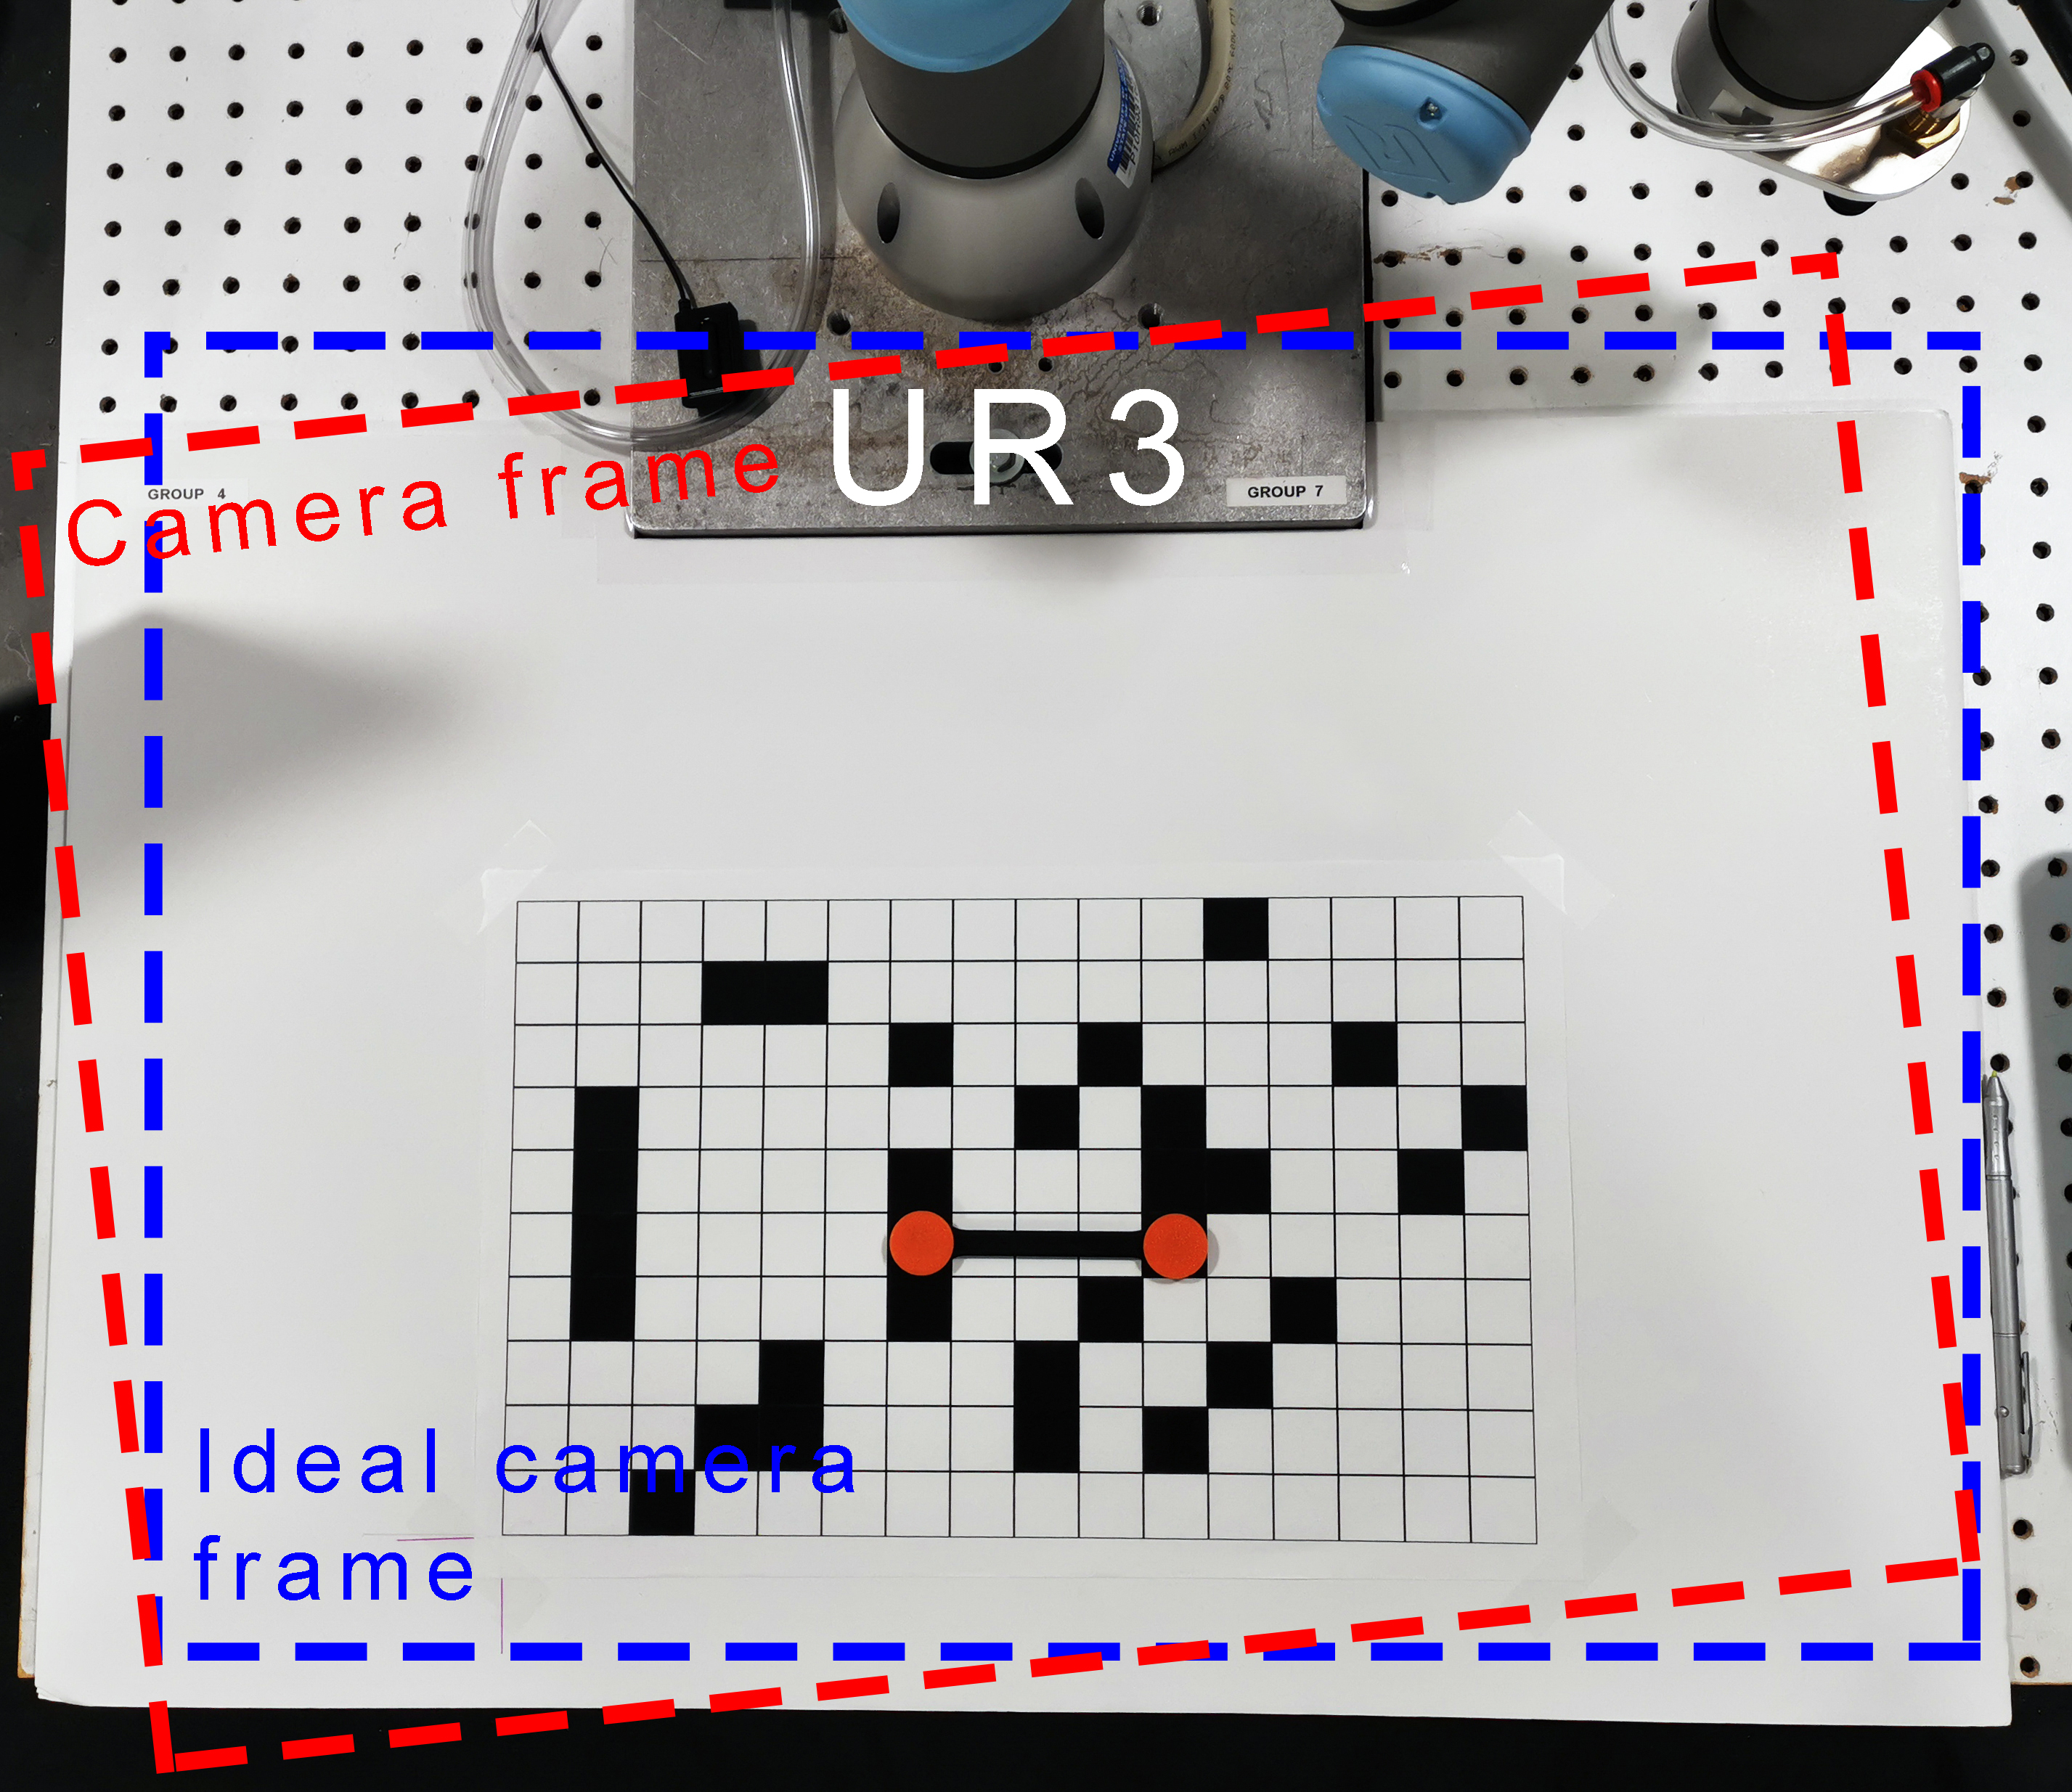
\includegraphics[height=5.5cm]{lab3_cam_cali2.jpg}	&  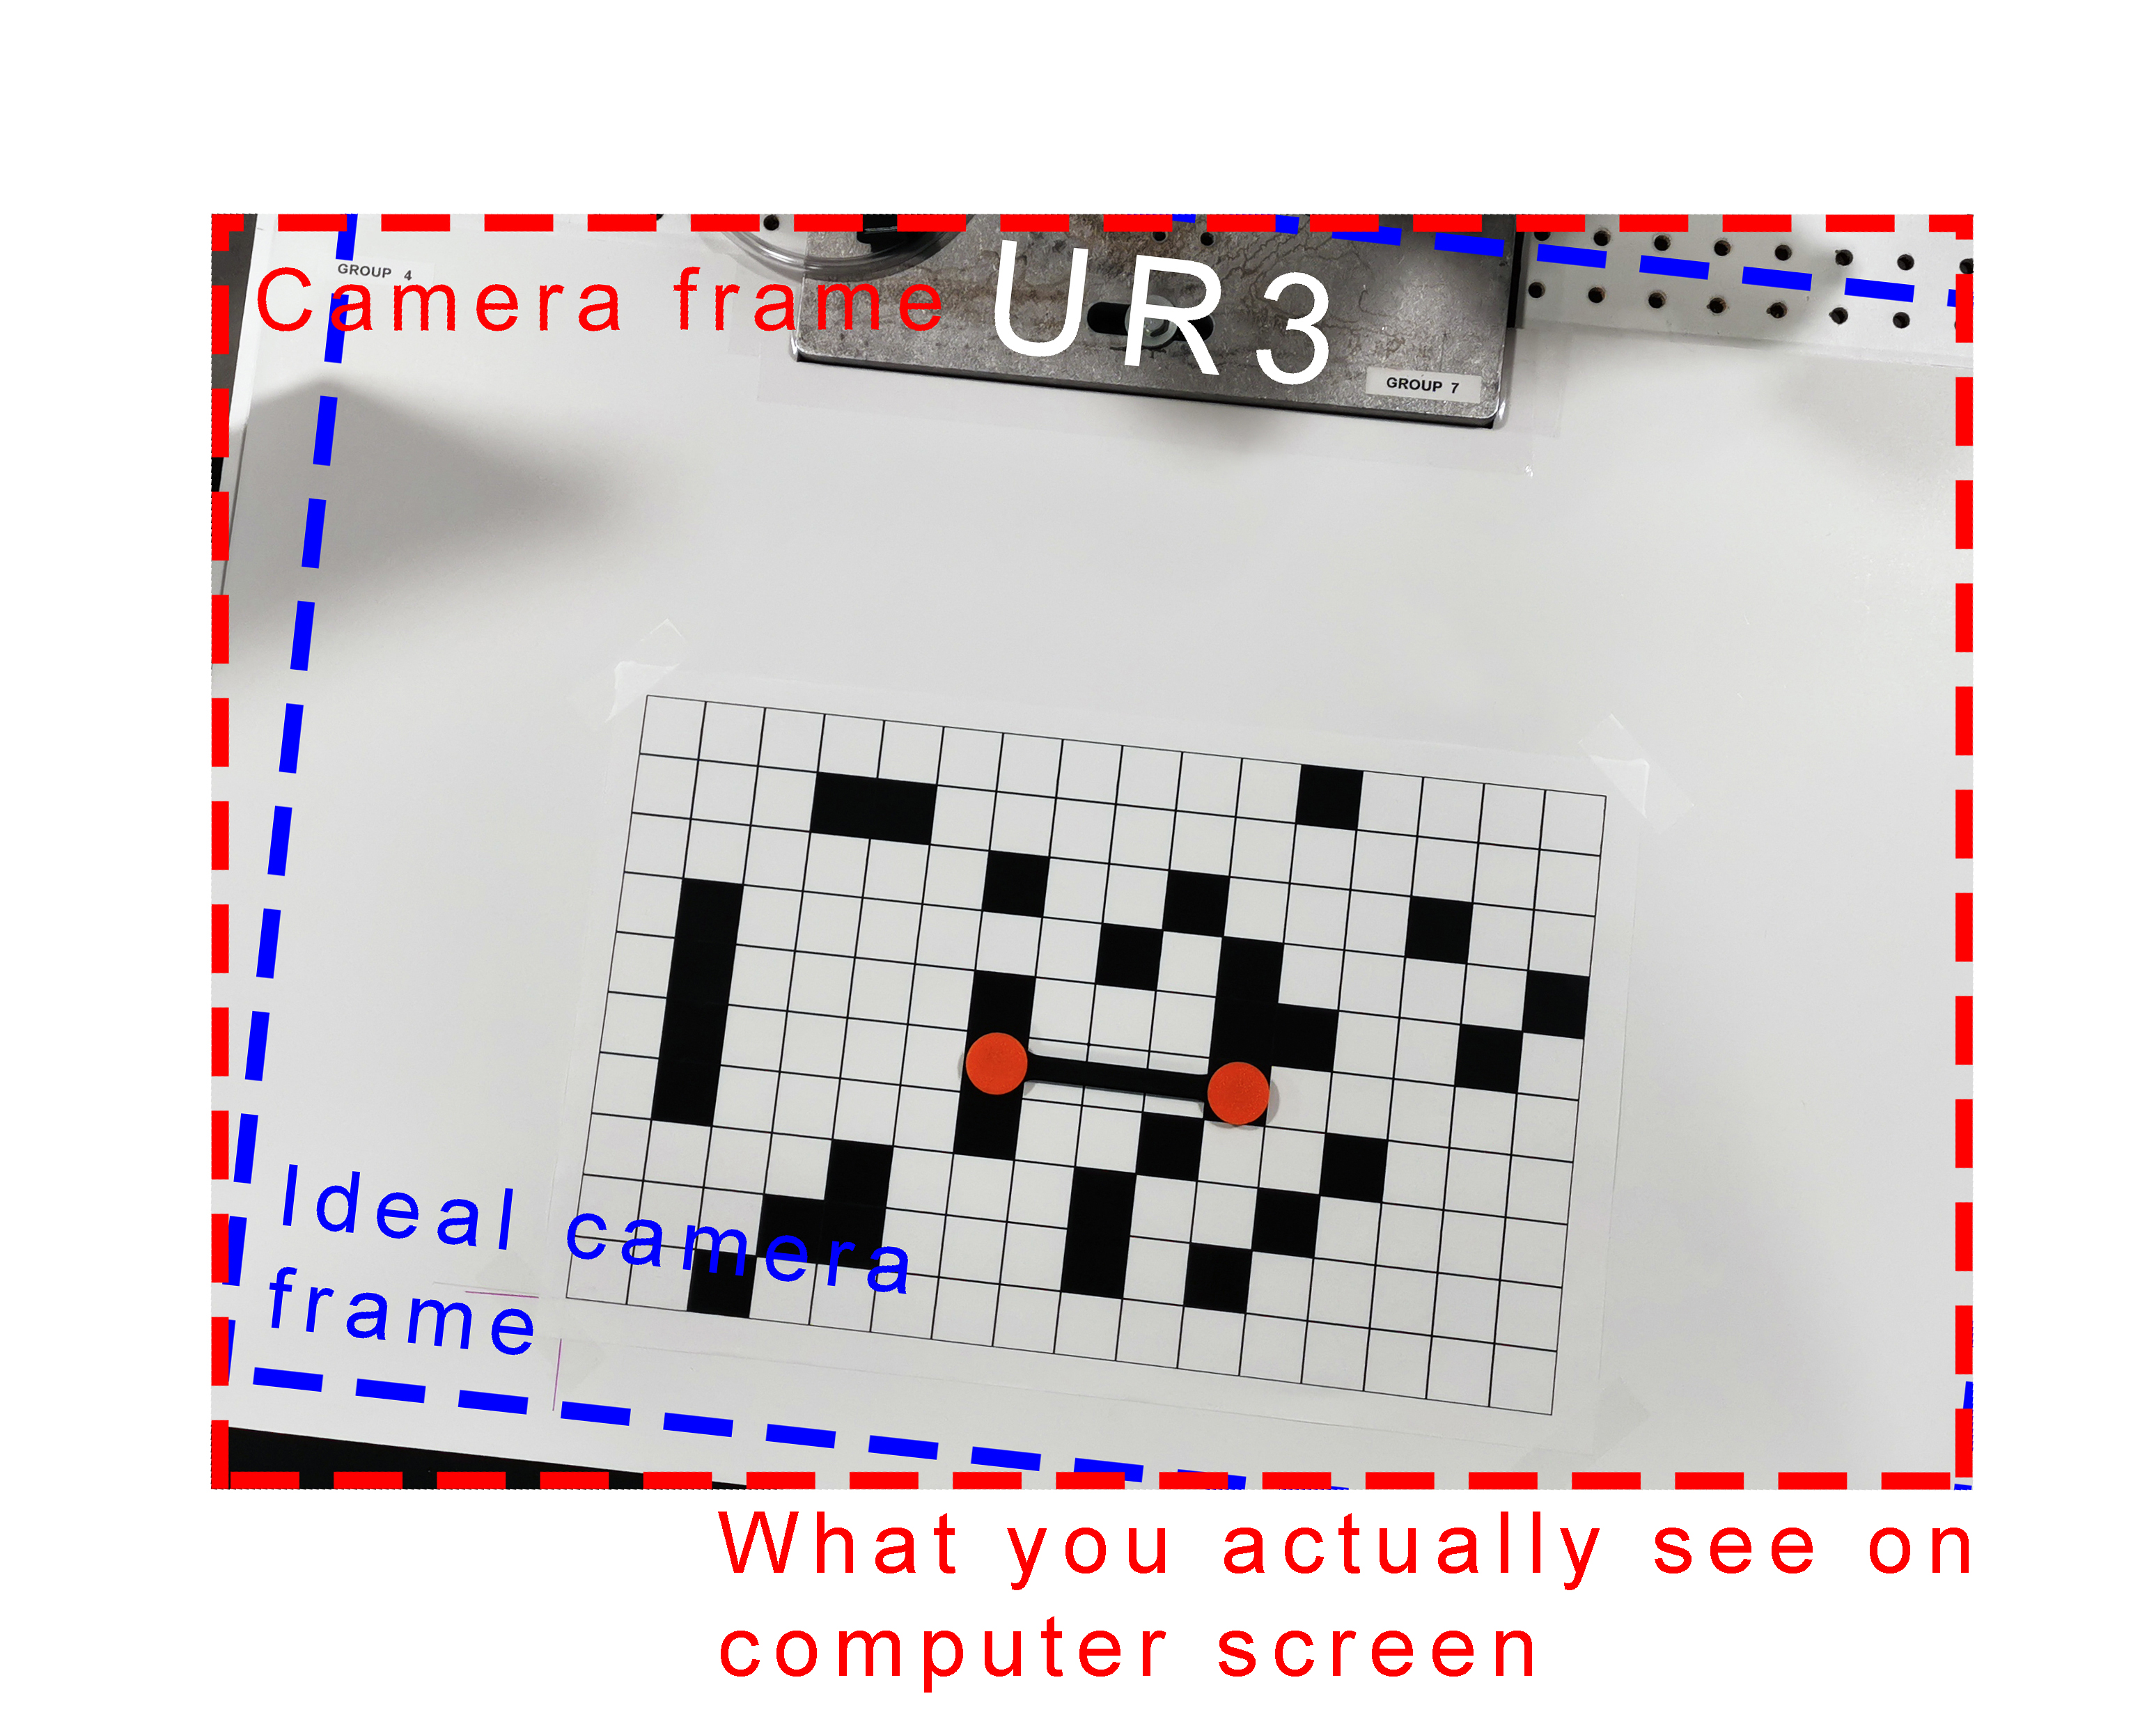
\includegraphics[height=5cm]{lab3_cam_cali3.jpg} \\
		(a) & (b)\\
	\end{tabular}
	\caption{\figlbl{3cali2} (a) Overhead view of the table; the rectangle delineated by blue dashed lines represents the desired camera's field of view, while the red dashed lines represents the actual camera's field of view  (b) The actual image seen by the camera.  Notice that $x_c$ increases with increasing row values, and $y_c$ increases with increasing column values.}
    \end{figure}

	$\theta$ is the angle of rotation between the world frame and the camera frame. \figref{3cali2} gives an overhead view of the blocks with a hypothetical cutout representing the image captured by the camera.  Because the camera's x and y axes are not quite parallel to the world x and y axes, the blocks appear rotated in the image. You may expect this parameter to be fairly small.

	\[
	\theta = 
	\]
	
	$T_x, T_y$ (unit in meters), the origin of the world frame expressed in the camera frame. 
	
	Substitute these values into the two equations you derived in step 2 above and solve for the unknown values.
	\begin{eqnarray*}
		T_x & = & \\
		T_y & = & 	
	\end{eqnarray*}
	
	These values will be copied into your lab6 code in the next section.
\end{enumerate}

\subsection{Pick and Place} \label{PickPlace}

Now that you have the camera setup and the values for $\beta$, $\theta$, $T_x$ and $T_y$ you are ready to start modifying the starter code for Lab 6. 

\begin{itemize}

\item Download the starter code from the website and add it to your catkin directory. Take a look at the four given Python files: \textbf{lab6\_header.py}, \textbf{blob\_search.py}, \textbf{lab6\_func.py} and \textbf{lab6\_exec.py}. 

\item \textbf{Lab6\_header.py}:  This file does not need to be changed.  It just includes items needed for this application.  If you would like to add other Python features you can of course modify this file.

\item \textbf{Lab6\_func.py}:  You will need to copy into this file work you have done in Labs 4 and 5.  \textbf{Get\_MS()}, \textbf{lab\_fk()} and \textbf{lab\_invk()} are all functions that you created in those previous labs.  You will use some or all of these functions to move the UR3 from one $X,Y,Z$ point to another point.

\item \textbf{Blob\_search.py}:  You will be modifying/adding code in this file.  The comments in this file will help you understand what you need to change.  You should notice that this file is very similar to the starter code given in Lab 3 to call the \textbf{SimpleBlobDetector} class. You will modify these functions to find the centroid of either bright green blocks or bright pink blocks depending on the value passed in the parameter “color”.  The \textbf{blob\_search()} function should return the world coordinates of the center of the colored blocks.  Make sure to change $\beta$, $\theta$, $T_x$ and $T_y$ to the values for your bench found in 6.5.3. 

\item \textbf{Lab6\_exec.py}:  You will need to add to this file.  The comments in this file are again helpful. \textbf{move\_block()} function will be similar to your \textbf{move\_block()} function in lab 2, but here you will be using inverse kinematics to figure out what thetas will bring the arm to the desired points. \textbf{Image\_callback()} is completed for you but make sure to understand what it is doing.  It is called each image of the video feed from the USB camera and finding the world coordinates of pink and green blocks and storing these coordinates to global variables so \textbf{main()} can access these variables. \textbf{main()} function has comments to show you where to add your code.  The initial code in \textbf{main()} starts the Publisher and Subscribers and then moves the robot arm out of the view of the camera.  Once the arm is out of the way it starts the video processing of the USB camera and sleeps for one second.  During that one second your vision processing code is run on each image and is finding the world coordinates of the pink and green blocks and storing the values to the global variables \textbf{xw\_yw\_R} and \textbf{xw\_yw\_G}.  The code you need to develop then takes the \textbf{xw\_yw\_R} variable and commands the robot to pick up the two pink blocks, one at a time, and place them in the “red area”.  Then using \textbf{xw\_yw\_G} place the two green blocks in the “green area”.  

\end{itemize}

\section{Report}
Each partner will submit a lab report using the guidelines given in the ECE 470: How to Write a Lab Report document.  Please be aware of the following:
\begin{itemize}
    \item Due to the end of semester, your TA will determine the due date for all Lab 6 requirements.  Note that late assignments are unlikely to be accepted.
    \item Lab reports will be submitted online at \href{https://www.gradescope.com}{GradeScope}.
\end{itemize}
Your lab report should include the following:
\begin{itemize}
    \item Explain how you performed blob detection and include any parameters that you set and how you set them.
    \item Give a brief overview of how your code achieves the goals of Lab 6.
    \item Explain how you you used the lessons from Labs 1 to 5 to achieve the goals of Lab 6.
    \begin{itemize}
        \item Explain what you learned and how it was used.
        \item Remember to be specific.
        \item A complete report should be able to include lessons from each lab.
    \end{itemize}
    
\end{itemize}
As appendices to your report, include the following:
\begin{itemize}
    \item Your $\textbf{lab6\_func.py}$ code 
    \item Your $\textbf{lab6\_exec.py}$ code
    \item Your $\textbf{Blob\_search.py}$ code
    \item Any other code that your wrote or edited
\end{itemize}


\section{Demo}
You will demonstrate to your TA your code which draws crosshairs over the centroid of each object in an image and reports the centroid coordinates 
in (row,column) and $(x,y)_w$ coordinates.  The robot should place the pink blocks in the ``pink block'' locations and the green blocks in the ``green block'' locations.

\section{Grading}
\begin{itemize}
\item 10 points, by the end of the first two hour lab session, show your TA that you have finished section \ref{ObjCentriod} and have started work on
section \ref{CamCal}.
\item 10 points, by the end of the second two hour lab session, show your TA that you have finished section \ref{CamCal} and have made good progress on
section \ref{PickPlace}.
\item 60 points, successful demonstration.
\item 20 points, report.
\end{itemize}